\chapter{State of the Art}

\section{Introduction}
This chapter reviews the current state of the art related to the design and
implementation of real-time Big Data platforms for IoT. It presents the
challenges associated with IoT data, the main architectural paradigms, the
technologies most commonly used in the literature and industry, as well as
the integration of artificial intelligence models for predictive analytics
and data enrichment. The goal is to position the proposed project within
the broader technological landscape.

\section{Fundamental Concepts}
\subsection{The emergence Big Data}
With the exponential growth of data, the concept of \textbf{Big Data} has
emerged, leading to the adoption of new techniques and technologies to manage
and analyze these massive volumes of information. The three main
characteristics, known as the \textbf{``5 Vs''}, illustrated below, define the
core aspects of Big Data:
\begin{itemize}
    \item \textbf{Volume:} Refers to the massive amount of data generated every second from various sources such as sensors, social networks, connected devices, and enterprise systems. Traditional data processing tools are not sufficient to handle such large datasets.
    
    \item \textbf{Velocity:} Describes the speed at which data is generated, collected, and processed. In the context of IoT, data streams arrive continuously in real-time, requiring fast ingestion and processing systems.
    
    \item \textbf{Variety:} Data comes in multiple formats and structures: structured (databases), semi-structured (JSON, XML), and unstructured (text, images, videos, sensor logs). This heterogeneity adds complexity to storage and analysis.
    
    \item \textbf{Veracity:} Refers to the quality, reliability, and accuracy of the data. In real world scenarios, data may be incomplete, inconsistent, or noisy, which can affect the reliability of the analysis.
    
    \item \textbf{Value:} The ultimate goal of Big Data is to extract meaningful insights and create added value. Without value extraction, data remains a cost rather than a strategic resource.
\end{itemize}

\begin{figure}[h!]
    \centering
    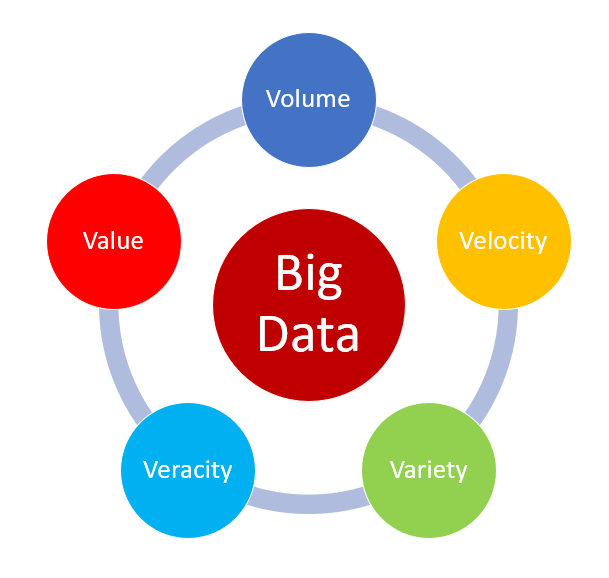
\includegraphics[width=0.4\textwidth]{images/5vs.png}
    \caption{the 5 V's of big data}
\end{figure}

\subsection{Big Data Paradigms and Architectures}

Big Data processing relies on two main paradigms: \textbf{batch processing} and \textbf{stream processing}. 

\begin{itemize}
    \item \textbf{Batch Processing:} Operates on large volumes of data collected over a period of time. A typical example is \textit{MapReduce}, which processes static datasets in multiple stages. Frameworks such as \textit{Apache Spark} extend this model by offering in memory computation for faster execution. Batch processing is well suited for tasks like log analysis or data aggregation where real time results are not required.
\begin{figure}[h!]
    \centering
    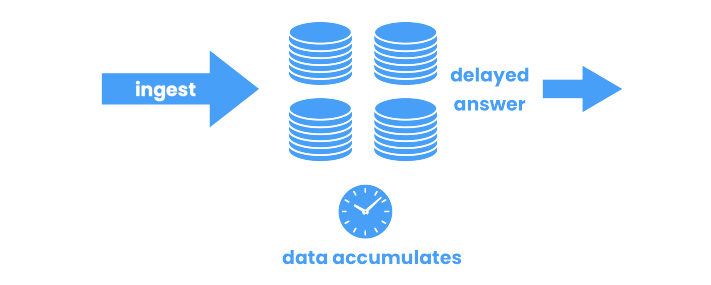
\includegraphics[width=0.6\textwidth]{images/databatch.png}
    \caption{Batch Processing}
\end{figure}
    \item \textbf{Stream Processing:} Focuses on continuous data flows, processing records as they arrive with low latency. Systems like \textit{Apache Flink} or \textit{Kafka Streams} provide event-driven architectures capable of handling high throughput, real time data streams. This approach is crucial in IoT contexts where immediate insights are needed (e.g., anomaly detection, predictive maintenance).
\end{itemize}
    \begin{figure}[H]
    \centering
    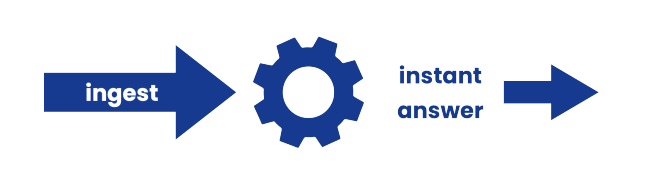
\includegraphics[width=0.6\textwidth]{images/dataStream.png}
    \caption{Stream Processing}
\end{figure}


To manage these paradigms, several architectural models have been proposed:

\begin{itemize}
    \item \textbf{Lambda Architecture:} Combines batch and real-time processing. The \textit{batch layer} ensures accuracy by computing views on historical data, while the \textit{speed layer} provides low-latency updates. A serving layer unifies the results. Although powerful, this model introduces complexity due to the dual maintenance of batch and stream pipelines.
    \end{itemize}
    \begin{figure}[H]
    \centering
    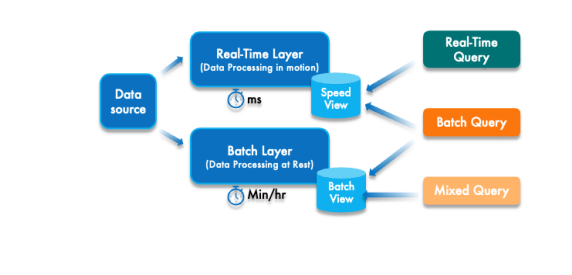
\includegraphics[width=0.6\textwidth]{images/lambda.png}
    \caption{Lambda Architecture}
\end{figure}
\begin{itemize}

    \item \textbf{Kappa Architecture:} Simplifies the Lambda model by removing the batch layer. All data is processed as a stream, using technologies like Kafka and Flink. Reprocessing is achieved by replaying historical events through the streaming pipeline. This makes the architecture more agile and better adapted to IoT and real-time analytics scenarios.

\end{itemize}
    \begin{figure}[H]
    \centering
    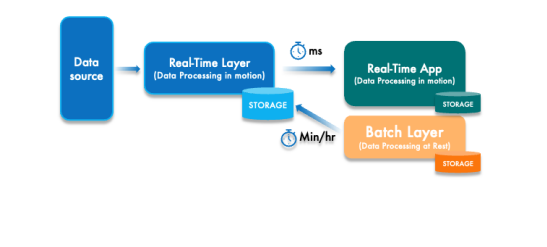
\includegraphics[width=0.6\textwidth]{images/kappa.png}
    \caption{Kappa Architecture}
\end{figure}

To better understand the differences between the two main architectures for big data stream processing, the following table summarizes the key characteristics of \textbf{Lambda} and \textbf{Kappa} architectures, highlighting their advantages, complexity, and typical use cases.

\begin{table}[h!]
    \centering
    \begin{tabular}{|p{4cm}|p{5cm}|p{5cm}|}
        \hline
        \textbf{Aspect} & \textbf{Lambda Architecture} & \textbf{Kappa Architecture} \\
        \hline
        Processing Model & Dual pipeline: batch layer + speed layer & Single pipeline: stream-only \\
        \hline
        Complexity & High, due to maintaining separate batch and stream layers & Lower, simpler design with only a stream layer \\
        \hline
        Data Reprocessing & Batch layer handles historical data; speed layer handles new events & Reprocessing is done by replaying events through the stream pipeline \\
        \hline
        Latency & Low latency real time layer + accurate batch results & Low latency only; relies on stream processing for all data \\
        \hline
        Use Cases & Scenarios where both historical accuracy and real time insights are needed & Real time analytics, IoT streaming, simpler operational requirements \\
        \hline
        Maintenance & More complex due to dual pipelines & Simpler; only one pipeline to maintain \\
        \hline
    \end{tabular}
    \caption{Comparison of Lambda and Kappa Architectures}
    \label{tab:lambda_kappa}
\end{table}

\subsection{Internet of Things (IoT)}

The \textbf{Internet of Things (IoT)} refers to a network of interconnected devices and sensors that collect, exchange, and act on data. IoT generates massive amounts of real time, heterogeneous data, which often require Big Data technologies for storage, processing, and analysis. Examples include smart factories, connected vehicles, and environmental monitoring systems.
\begin{figure}[H]
    \centering
    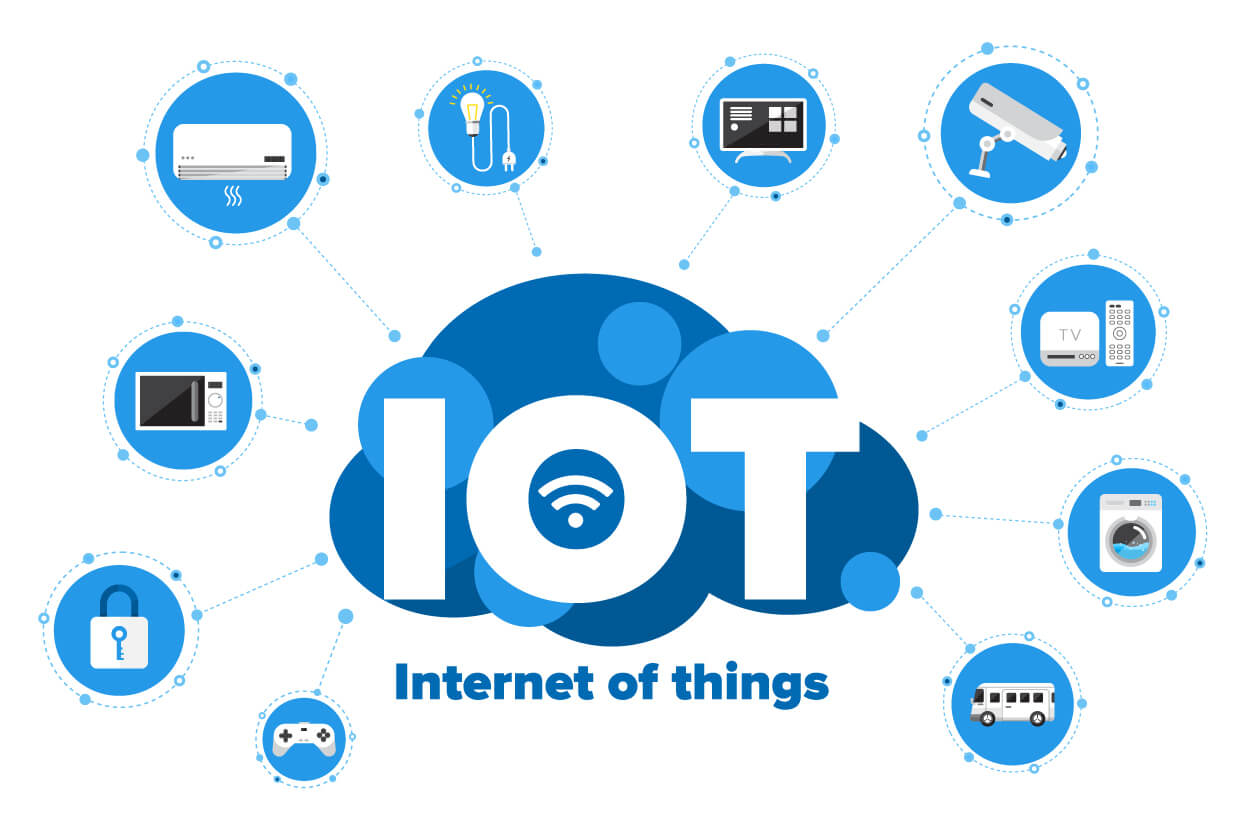
\includegraphics[width=0.6\textwidth]{images/IoT.jpg}
    \caption{IoT }
\end{figure}


\subsection{Infrastructure for Big Data}

A robust infrastructure is fundamental for supporting large scale, real time IoT data processing. It provides the foundation on which all data pipelines, analytics, and AI models operate. Modern Big Data infrastructures rely on automation, orchestration, and containerization to ensure scalability, reliability, and maintainability.

Automation tools allow the infrastructure to be deployed and configured consistently across different environments, reducing human errors and accelerating setup times. Orchestration platforms manage the deployment, scaling, and lifecycle of services, ensuring that applications run efficiently under varying workloads. Containerization provides isolated, reproducible environments for applications, enabling seamless updates, portability, and resource optimization.

Together, these concepts allow a Big Data platform to handle high throughput data streams, adapt dynamically to changing demands, and maintain operational stability, which is essential for real time IoT applications.


\subsection{Predictive and Generative Analytics}

Big Data platforms can leverage \textbf{AI and Machine Learning} to extract actionable insights:

\begin{itemize}
     \item \textbf{Predictive Analytics:}  
    Predictive analytics uses historical and real-time data to forecast future events, trends, or behaviors. In the context of IoT and Big Data, models such as \textit{LSTM} (Long Short-Term Memory) and \textit{GRU} (Gated Recurrent Unit) are particularly effective for analyzing sequential or time-series data generated by sensors. These models can identify patterns and anomalies in the data, enabling early detection of potential equipment failures, performance degradation, or operational inefficiencies. By leveraging predictive analytics, organizations can implement proactive maintenance strategies, reduce downtime, optimize resource usage, and make more informed decisions based on anticipated events rather than reactive responses.
    
   \item \textbf{Data Augmentation:}  
    Data augmentation involves artificially increasing the size and diversity of a dataset to improve the performance of machine learning models. Generative models, such as \textit{GANs} (Generative Adversarial Networks), are commonly used for this purpose in Big Data and IoT contexts. GANs generate realistic synthetic data that mimics the statistical properties of the original dataset, allowing models to train on a richer and more varied set of examples. This process helps to mitigate issues such as class imbalance, limited data availability, or noise in the data, ultimately enhancing the accuracy, generalization, and robustness of predictive models, particularly in applications like predictive maintenance, anomaly detection, and forecasting.
\end{itemize}

\section{Industry Examples of Big Data Platforms}

Several leading companies have successfully implemented Big Data solutions to handle massive, real-time data streams. Here are some illustrative examples:

\subsubsection{Tesla}
Tesla leverages Big Data to optimize its electric vehicles and autonomous driving systems. Sensor data from cars is collected in real time and sent to centralized platforms for analysis. The company uses cloud-based storage, streaming technologies, and AI models to process telemetry, driving behavior, and predictive maintenance. Tesla’s architecture follows a \textbf{Kappa-like stream processing model} for real-time analytics, combined with batch processing for historical insight.

\begin{figure}[H]
    \centering
    
\includegraphics[width=0.3\textwidth]{images/Tesla_logo.png}
    \caption{Tesla logo}
\end{figure}

\subsubsection{Amazon}
Amazon relies heavily on Big Data to manage e-commerce operations, recommendations, and logistics. The company uses a combination of \textit{Hadoop}, \textit{Spark}, and \textit{AWS cloud services} for scalable storage and processing. Real-time inventory and user activity are handled using streaming frameworks like \textit{Kafka} and \textit{Flink}. Amazon typically employs a \textbf{Lambda architecture} to combine batch processing for historical analytics and stream processing for real-time recommendations and operational decisions.

\begin{figure}[H]
    \centering
    
\includegraphics[width=0.3\textwidth]{images/Amazon_logo.svg.png}
    \caption{Amazon logo }
\end{figure}

\subsubsection{Uber}
Uber processes high-frequency trip, GPS, and user data to provide dynamic pricing, route optimization, and predictive demand management. The platform uses \textit{Kafka} for ingestion, \textit{Hadoop} and \textit{Spark} for batch processing, and \textit{Flink} for real-time stream processing. Uber’s data architecture is largely inspired by the \textbf{Lambda architecture}, integrating both batch and stream layers 
to ensure accuracy and low-latency decision making.

\begin{figure}[H]
    \centering
    
\includegraphics[width=0.3\textwidth]{images/Uber_logo_2018.png}
    \caption{Uber logo }
\end{figure}

These examples illustrate how global companies adapt Big Data architectures and technologies to manage IoT and real-time data, optimize operations, and extract actionable insights.

\section{Conclusion}

This chapter outlined the key concepts and paradigms of Big Data for IoT, from the ``5Vs'' to batch and stream processing, as well as the Lambda and Kappa architectures. We also highlighted the importance of infrastructure and the role of AI models in predictive and generative analytics. Finally, industry examples from Tesla, Amazon, and Uber illustrated how these technologies are applied in practice, positioning the proposed project within this technological landscape.







